
%-----------------------------------------------------------------------------
\chapter{A program for annotating and predicting the
effects of single nucleotide polymorphisms,
SnpEff: SNPs in the genome of Drosophila
melanogaster strain $w^{1118}$ ; iso-2; iso-3\label{ch:snpeff}}
%-----------------------------------------------------------------------------

%---
\section{Preface}
%---

As this thesis is focused on extracting biological insight from sequencing data, in this chapter we examine algorithms we created for calculating ``functional annotations" of genomic variants. In essence, functional variant annotations are bits of biological knowledge that allow us to make prioritize variants that are assumed to be more relevant to the phenotypic trait under study and to filter out variants assumed irrelevant. The spectrum of functional annotations for a genomic variant is wide and may involve information on which genes are affected by the variant, how the protein product is affected, how conserved is the genomic region the variant lies onto, and which clinically relevant information is associated with the loci; just to mention a few typical use cases.

When trying to find variants that affect risk of complex disease, statistical power is paramount. We need to be able to ``separate wheat from chaff". In our context this means two different but closely related tasks: i) performing functional annotations, and ii) using that information for prioritizing variants (and filtering out the ones we suspect are not related to the particular trait under study). Failing to efficiently filter out irrelevant variants would reduce our statistical power as more statistical tests are calculated, thus would decrease our chances of finding the associations we are looking for. In order to efficiently annotate and filter variants, we created two software packages called SnpEff and SnpSift that deal with the annotation and filtering aspects respectively.

The rest of the chapter is published in: Cingolani, Pablo, Rob Sladek, and Mathieu Blanchette. ``BigDataScript: a scripting language for data pipelines." Bioinformatics 31.1 (2015): 10-16.

%---
\section{Abstract}
%---

We describe a new computer program, SnpEff, for rapidly categorizing the effects of single nucleotide polymorphisms (SNPs) and other variants such as multiple nucleotide polymorphism (MNPs) and insertion-deletions (InDels), in whole genome sequences. Once a genome is sequenced, the SnpEff program can be used to annotate and classify genetic polymorphisms based on their effects on annotated genes, such as synonymous or non-synonymous SNPs, start codon gains or losses, stop codon gains or losses; or based on their genomic locations, such as intronic, 5' untranslated region (5' UTR), 3' UTR, upstream, downstream or intergenic regions. Here the use of SnpEff is illustrated by annotating \~356,660 candidate SNPs in \~117 Mb unique sequences, representing a substitution rate of \~1/305 nucleotides, between the Drosophila melanogaster $w^{1118}$ ; iso-2; iso-3 strain and the reference y 1 ; cn 1 bw 1 sp 1 strain. We show that \~15,842 SNPs are synonymous and \~4,467 SNPs are non-synonymous (N/S \~0.28) and the remainder are in other categories, such as stop codon gains (38 SNPs), stop codon losses (8 SNPs) and start codon gains (297 SNPs) in the 5' UTR. We found, as expected, that the SNP frequency is proportional to the recombination frequency (i.e., highest in the middle of chromosome arms).  We also found that start-gained and stop-lost SNPs in Drosophila melanogaster often encode N-terminal and C-terminal amino acids that are conserved in other Drosophila species. This suggests that the 5' and 3' UTRs are reservoirs of cryptic genetic variation that can be used multiple times during the evolution of the Drosophila genus. At this time, SnpEff has been set up for annotating DNA polymorphisms of over 320 genome versions of multiple species including the human genome. It has already been used by over 50 institutions and universities in the bioinformatics community. Tools such as SnpEff are valuable because, as sequencing becomes cheaper and more available, whole genome sequencing is becoming more important in model organism genetics.

%---
\section{Introduction}
%---

When we re-sequenced the $w^{1118}$ ; iso-2; iso-3 genome in 2009, 1 bioinformatics tools available then were unable to rapidly catego- rize the \~356,660 SNPs as comparing to the y 1 ; cn 1 bw 1 sp 1 refer- ence strain. At the time, other available tools such as ENSEMBL’s variant web application (http://ensembl.org) could only analyze a few hundred to a few thousand SNPs per batch. Therefore, over the past couple of years, we have been developing a new program, SnpEff, which is able to analyze and annotate thousands of variants per second. In addition to SnpEff, other programs to annotate genomic variants are currently now available, such as Annotate Variation (ANNOVAR) 2 and Variant Annotation, Analysis and Search Tool (VAAST). 3 However, SnpEff supports more genome versions, is open source for any user, supports variant call format (VCF) files and it is marginally faster (although the speeds of SnpEff, ANNOVAR and VAAST are comparable). Table S1 shows a feature comparison of some currently available software packages.

SnpEff, an abbreviation of ``SNP effect," is a multi-platform open source variant effect predictor program. SnpEff annotates variants and predicts the coding effects of genetic variations, such as SNPs, insertions and deletions (INDELs) and multiple nucleotide polymorphisms (MNPs) (http://SnpEff.sourceforge.net/).  The main features of SnpEff include: (1) speed—the ability to make thousands of predictions per second; (2) flexibility—the ability to add custom genomes and annotations; (3) the ability to integrate with Galaxy, an open access and web-based platform for computational bioinformatic research (http://gmod.org/wiki/ Galaxy); (4) compatibility with multiple species and multiple codon usage tables (e.g., mitochondrial genomes); (5) integration with Genome Analysis Toolkit (GATK); 4 and (6) ability to perform non-coding annotations. When SnpEff was integrated into the GATK, it replaced the ANNOVAR program for variant analyses.

\begin{figure}
    \centering
    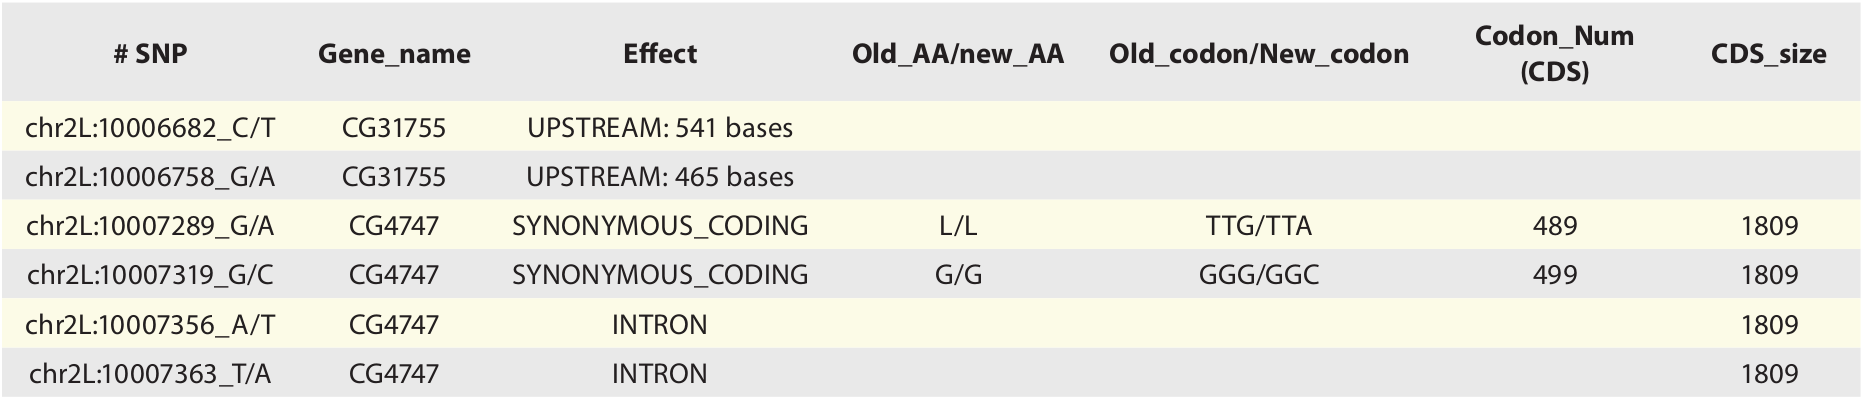
\includegraphics[width=14cm]{snpeff_table1.png}
    \caption{Output of SnpEff.\# SNP, a description of the single nucleotide polymorphism (SNP) indicating chromosome arm (chr2L), coordinate in genome (10006682), and nucleotide change (e.g., C/T indicates that C is replaced by T in $w^{1118}$ ; iso-2; iso-3 at this position). Gene\_name, official gene symbol of gene. Effect, description of SNP (e.g., upstream of transcription start site at position 541). Old\_AA/new\_AA, amino acid change, if any, in one letter code. Old\_codon/New\_codon, if a codon contains a SNP, the old (reference) and new ($w^{1118}$ ; iso-2; iso-3) codons are indicated. Codon\_Num (CDS), the codon number of the coding sequence (CDS). CDS\_size, the size of the protein in amino acids.}
    \label{fig:snpeffTab1}
\end{figure}

A simple walk-through example on how to analyze sequencing data to calculate variants and their effects is shown in Listing SL1. This example is intended for illustration purposes only since many additional steps are routinely used in re-sequencing data analysis pipelines, but design of a fully featured pipeline is beyond the scope of this paper.

Here, we report the results of SnpEff (version 1.9.6) analyses of the \~356,660 candidate SNPs that we identified in $w^{1118}$ ; iso-2; iso-3 with respect to the y 1 ; cn 1 bw 1 sp 1 reference strain as reported in our previous paper. 1 This is of great interest to the Drosophila community because thousands of transposon insertion stocks 5 and hundreds of deficiency stocks 6,7 were generated in the $w^{1118}$ ; iso-2; iso-3 genetic background. The large number and potential severity of many SNPs in the two laboratory strains was a surprising finding, and the possible evolutionary implications of this finding are discussed.

%---
\section{Results}
%---

\textbf{Formats used in SnpEff.} To understand the potential effects of large numbers of SNPs in genome sequence comparisons, we developed an open-source tool, SNPeff, to classify SNPs based on gene annotations. Table 1 shows the beginning portion of the output generated by SnpEff when the SNPs in $w^{1118}$ ; iso-2; iso-3 were compared with the reference genome, y 1 ; cn 1 bw 1 sp 1 that is represented in Drosophila melanogaster release 5.3. A more complete SnpEff effect list is shown in Table 2. Before using SnpEff, an input file must be generated that lists all of the SNPs and INDELs in a genome. We published the input file for $w^{1118}$ ; iso-2; iso-3 in our previous paper, 1 and it was derived by comparing hundreds of millions of short sequence reads (\~20-fold genome coverage) and identifying SNPs based on a Sequence Alignment/Map tools (SAMtools) quality score for each nucleotide in the genome. 8

Input formats supported by SnpEff are variant call format (VCF), 9 tab separated TXT format; and and the SAMtools

Pileup format. 8 VCF was created by the 1,000 Genomes project and it is currently the de facto standard for variants in sequencing applications. The TXT and Pileup formats are currently deprecated and being phased out.

SnpEff also supports two output formats, TXT and VCF. The information provided in both of them includes four main groups: (i) variant information (genomic position, the reference and variant sequences, change type, heterozygosity, quality and coverage); (ii) genetic information (gene Id, gene name, gene biotype, transcript ID, exon ID, exon rank); and (iii) effect information (effect type, amino acid changes, codon changes, codon number in CDS, codon degeneracy, etc.).

Whenever multiple transcripts for a gene exist, the effect and annotations on each transcript are reported, so one variant can have multiple output lines. Table 3 shows the information provided by each column in TXT format and Table 4 shows the information provided in VCF format. When using VCF format, the effect information is added to the information (INFO) fields using an effect (EFF) tag. As in the case of TXT output, if multiple alternative splicing products are annotated for a particular gene, SnpEff provides this information for each annotated version (see Sup. Data File 1 for the complete SnpEff output for $w^{1118}$ ; iso-2; iso-3).

Predicted effects are with respect to protein coding genes.  Variants affecting non-coding genes are annotated and the corresponding biotype is identified, whenever the information is available. A ``biotype" is a group of organisms having the same specific genotype.

According to SnpEff (version 1.9.6), the largest number of SNPs in $w^{1118}$ ; iso-2; iso-3 are in introns (130,126) followed by those in upstream (76,155), downstream (71,645) and intergenic (51,783) regions (Fig. 1). ``Upstream" is defined as 5 kilobase (kb) upstream of the most distal transcription start site and ``downstream" is defined as 5 kb downstream of the most distal polyA addition site, but these default variables can be easily adjusted.  SnpEff also found thousands of SNPs within the exons. For example, there are 3,718 SNPs in the 3' untranslated regions (3' UTR) and 2,508 SNPs in the 5' untranslated regions (5' UTR).  The SNPs in the upstream, downstream, 5' and 3' UTR regions might affect transcription or translation, but the actual effects have to be confirmed case-by-case. In the next few sections, we present examples of several types of SNPs that might affect the protein function.

\begin{figure}
    \centering
    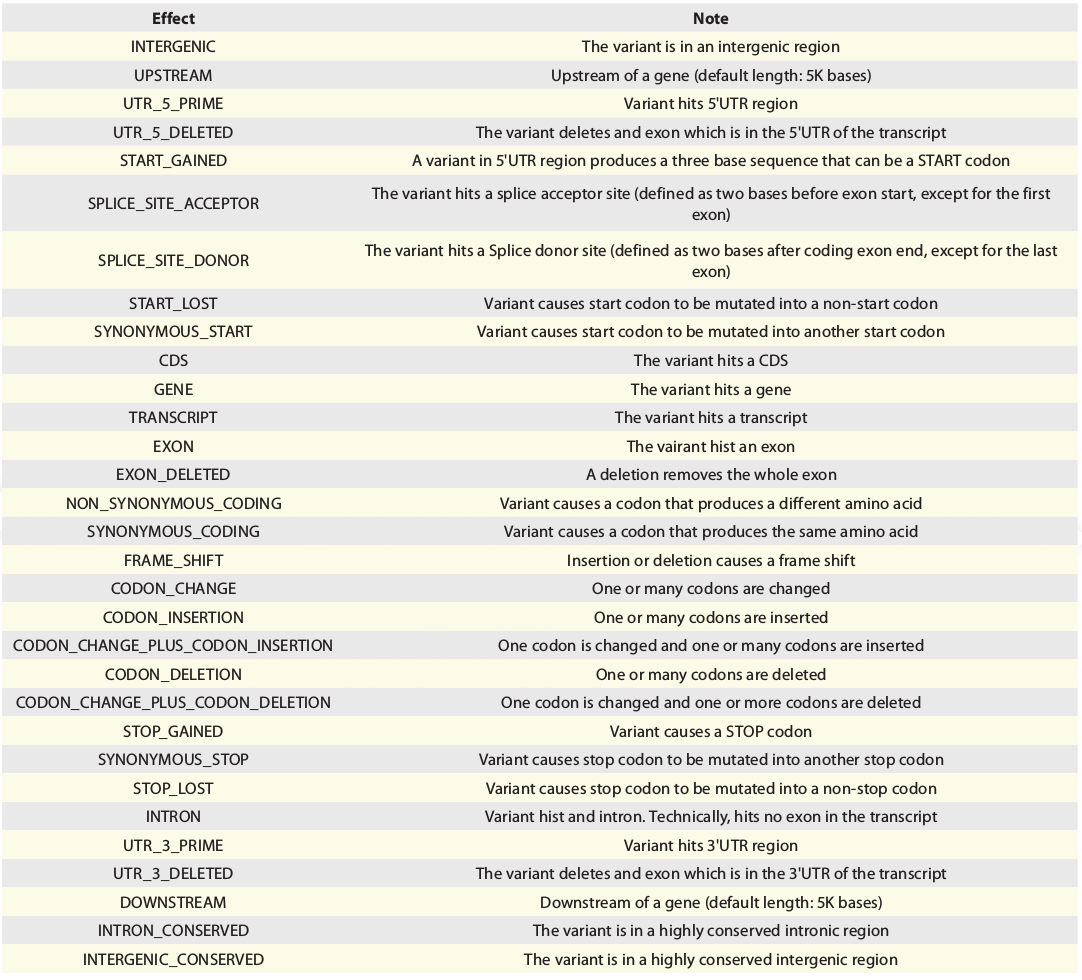
\includegraphics[width=14cm]{snpeff_table2.png}
    \caption{Detailed effect list from SnpEff}
    \label{fig:snpeffTab2}
\end{figure}

Heterozygosity is not considered in the $w^{1118}$ ; iso-2; iso-3 sequence because the stock was isogenized and only high quality (i.e., homozygous SNPs) were used for this analysis. 1 

The SnpEff website (http://snpeff.sourceforge.net/SnpSift.  html) has a frequently asked questions (FAQ) section that addresses most issues that a user might have in operating this program.

\textbf{SNPs that generate new start codons.} There are 297 SNPs that potentially generate a new translation initiation codon in the 5' UTR (start-gained SNPs). The most common translation initiation codon is AUG, which is coded by ATG in the genome.  To be thorough, we also included CUG and UUG codons, which code for leucine, as these codons can also be used to initiate translation in rare genes in Drosophila and mammals. 10,11 There are 60 genes with ATG start-gained SNPs (Table 5), 99 genes with CTG start-gained SNPs and 120 genes with TTG startgained SNPs in $w^{1118}$ ; iso-2; iso-3, all by definition in 5' UTR regions, compared with the reference genome (the reading frame is indicated on the SnpEff table). Most of the ATG start-gained SNPs are within 1 kb of the annotated translation start (Table 5), but this probably reflects the fact that most 5' UTR sequences are less than 1 kb long. Less than expected by chance, only \~25\% of the ATG start-gain SNPs are in the same reading frame as the annotated translation start point (Table 5). Since 33\% of in frame ATG start-gained SNPs are expected by chance, this suggests that there might be weak selection against this class of SNPs. Of the 60 genes with ATG start-gained SNPs, five genes have two ATG start-gained SNPs and one gene has three startgained SNPs; the remaining 54 genes have a single start-gained SNP. Since SnpEff does not take into account the Kozak consensus sequence flanking the AUG site, 5'-ACC AUG G-3', that is generally required for efficient translation, 12 and thus further assessment is required to determine whether a start-gained SNP is actually used.

\begin{figure}
    \centering
    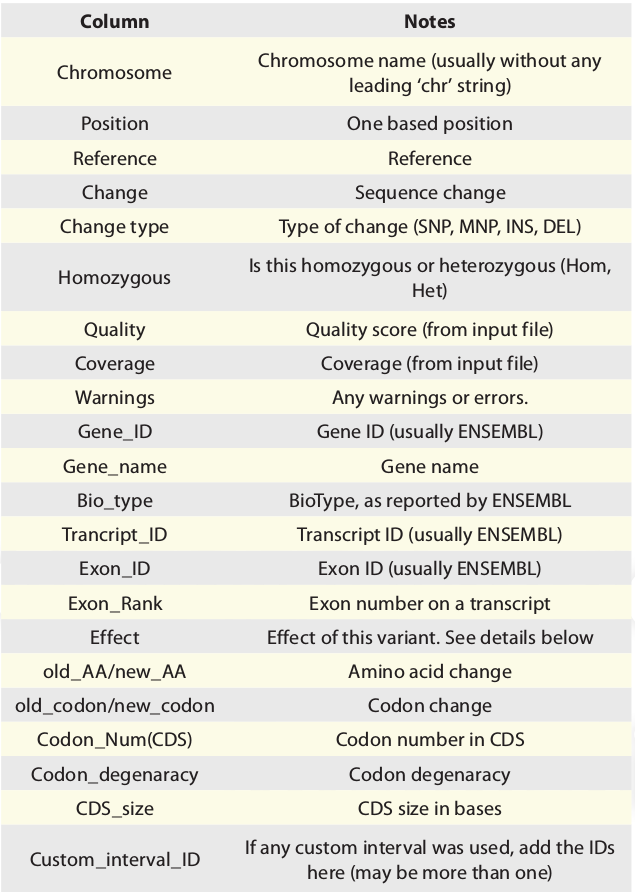
\includegraphics[width=8cm]{snpeff_table3.png}
    \caption{Information provided by SnpEff in tab separated output format
(TXT)}
    \label{fig:snpeffTab3}
\end{figure}


Gene ontology (GO) pathway analysis of the genes affected by the 297 start-gain SNPs in $w^{1118}$ ; iso-2; iso-3 was done using DAVID (Database for Annotation, Visualization and Integrated Discovery). 13,14 We found that the GO categories ``tissue morphogenesis," ``immunoglobulin like," ``developmental protein," and ``alternative splicing" are significantly enriched after multiplecomparisons correction by false-discovery rate (FDR < 0.001; Table 6). These categories are interesting because they predominantly contain proteins that show a wide degree of intra- and interspecies variability. For example, the immunoglobulin loci, which are highly divergent among humans and in other vertebrates, are used for antigen recognition. 15 Also, developmental proteins and proteins involved in tissue morphogenesis often have both conserved domains, such as the Hox domain, and highly divergent domains that maintain morphological diversity within a species, such as the trans-activation domains. 16,17

Our previous analyses suggest that most of the SNPs that we identified in $w^{1118}$ ; iso-2; iso-3 are probably genuine and can be validated by capillary sequencing. 1 A common worry about nextgeneration sequencing data in general is that SNPs are vastly over estimated. One might thing that if a large fraction of the identified SNPs had the predicted ``effects", the organism would not be viable. However, since short-read next-generation sequencing has a high error rate, such as the short-read sequences we obtained with the Illumina platform, further validation of specific SNPs is needed to be absolutely certain. Further validation of SNPs is best done with long-range DNA sequencing, such as with traditional capillary sequencing, or sequencing with the Roche, 18 and many other DNA sequencing instruments that are now available 20 (see ref.1 for validation examples with capillary sequencing).

An example of a start-gained SNP is found in the 5' UTR of Ecdysone inducible protein 63E (Eip63E) gene, which is predicted to be a cyclin J dependent kinase required for oogenesis and embryonic development (Fig. 2). 21 The potential start-gain SNP (A > G) in Eip63E changes 5'-ATA-3' to 5'-ATG-3' in the same reading frame with no in-frame intervening stop codons (Fig.  2A). If translation occurs at the new start-gained SNP, it would produce a protein with 57 additional N-terminal amino acids compared with the reference gene (Fig. 2B). However, the three bases prior to the new 5'-ATG-3' sequence, 5'-AAT-3', is a poor match to the Kozak consensus sequence, 5'-ACC-3', discussed above in reference 12. Therefore, it is unclear whether the startgain SNP in Eip63E is recognized by the ribosomal machinery.

It is interesting that a BLASTp search of the protein database reveals that the N-terminal 57 amino acids in Eip63E are 63\% identical (36/57) to the 58 N-terminal amino acids of the orthologous gene in Drosophila yakuba, but not to any other Drosophila species. D. yakuba is very close to D. melanogaster in the phylogeny. This suggests that the 5' UTR of Eip63E might be a source for cryptic genetic variation encoding novel N-terminal protein sequences that potentially modulates protein function (see Discussion).

\textbf{SNPs that generate new stop codons.} Another surprise in our SnpEff analysis was the identification of 28 stop-gained SNPs and 5 stop-lost SNPs in $w^{1118}$ ; iso-2; iso-3 (Table 7). A stop-gained SNP, classically called a nonsense SNP, has a coding codon changed to a stop codon, UAA, UAG, UGA. 22 Three genes, oc/ otd, LRP1 and trol9, have two stop-gained SNPs. Surprisingly at least 8 of the stop-gained SNPs are in genes that encode essential proteins, and these are Dif, dp, ex, MESR4, mew, oc/otd, tai and trol. It is not known whether the other stop-gained SNPs also affect essential protein-coding genes because their functions have not yet been characterized (according to www.flybase.org). We note that what would be a stop-gained SNP in $w^{1118}$ ; iso-2; iso-3 would be a stop-lost SNP in the reference strain, and vice versa, because the sequence of the ancestral Drosophila melanogaster strain that gave rise to both of these strains is not known.

An important consideration with stop-gained and stop-lost SNPs is whether the C-terminal amino acids in the longest version of the protein that not present in the shortest version of the protein are conserved in other Drosophila species. If the additional C-terminal amino acids are not conserved, then these amino acids might not affect the essential function of the protein but they might exert modulatory effects. If the additional C-terminal amino acids are conserved in multiple Drosophila species, then their loss might adversely affect the function of the protein. Therefore, in Table 7, we further classify the stop-gained and stop-lost SNPs into four categories: Category 1, including 23 genes, with both the N-terminal and novel C-terminal regions conserved among Drosophila species and other organisms; Category 2, including only one gene, with the entire gene sequence not conserved even among other Drosophila species; Category 3, with two genes, with the novel C-termini not conserved among other Drosophila species. In this category, the N-termini are conserved among Drosophila species, but this conservation is not maintained beyond the Drosophila genus (this class is likely a novel gene that arose in the Drosophila genus); and Category 4, including seven genes, with the novel C-terminal regions conserved among other Drosophila species but not beyond the Drosophila genus. In this category, the N-terminus is conserved beyond the Drosophila genus (this class probably has a C-terminal domain with a modulatory role in the Drosophila genus but not beyond the genus).

\begin{figure}
    \centering
    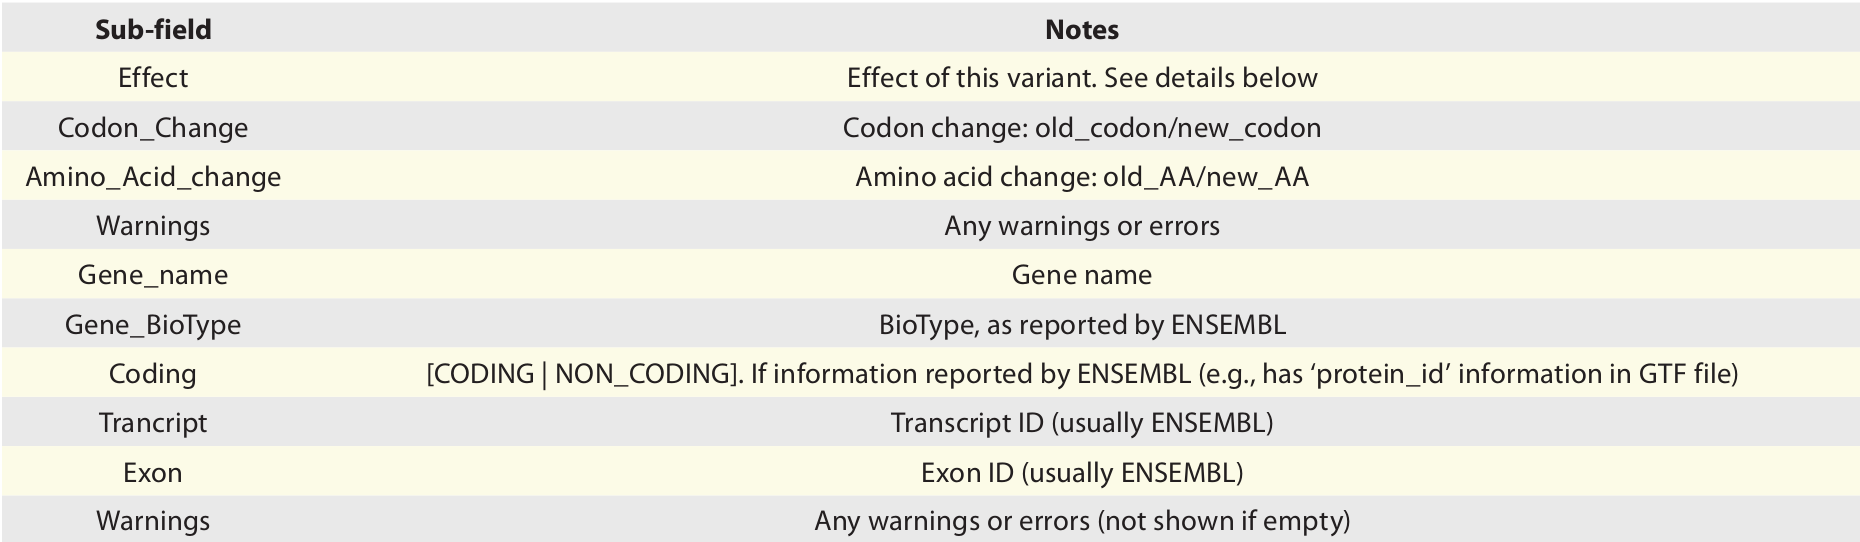
\includegraphics[width=14cm]{snpeff_table4.png}
    \caption{Information provided by SnpEff in variant call format (VCF). The information is added to the INFO fields using an tag 'EFF'. The format for each effect is ``\texttt{Effect (Effect\_Impact | Codon\_Change | Amino\_Acid\_change | Gene\_Name | Gene\_BioType | Coding | Transcript | Exon [ | ERRORS | WARNINGS ])}".}
    \label{fig:snpeffTab3}
\end{figure}

\begin{figure}
    \centering
    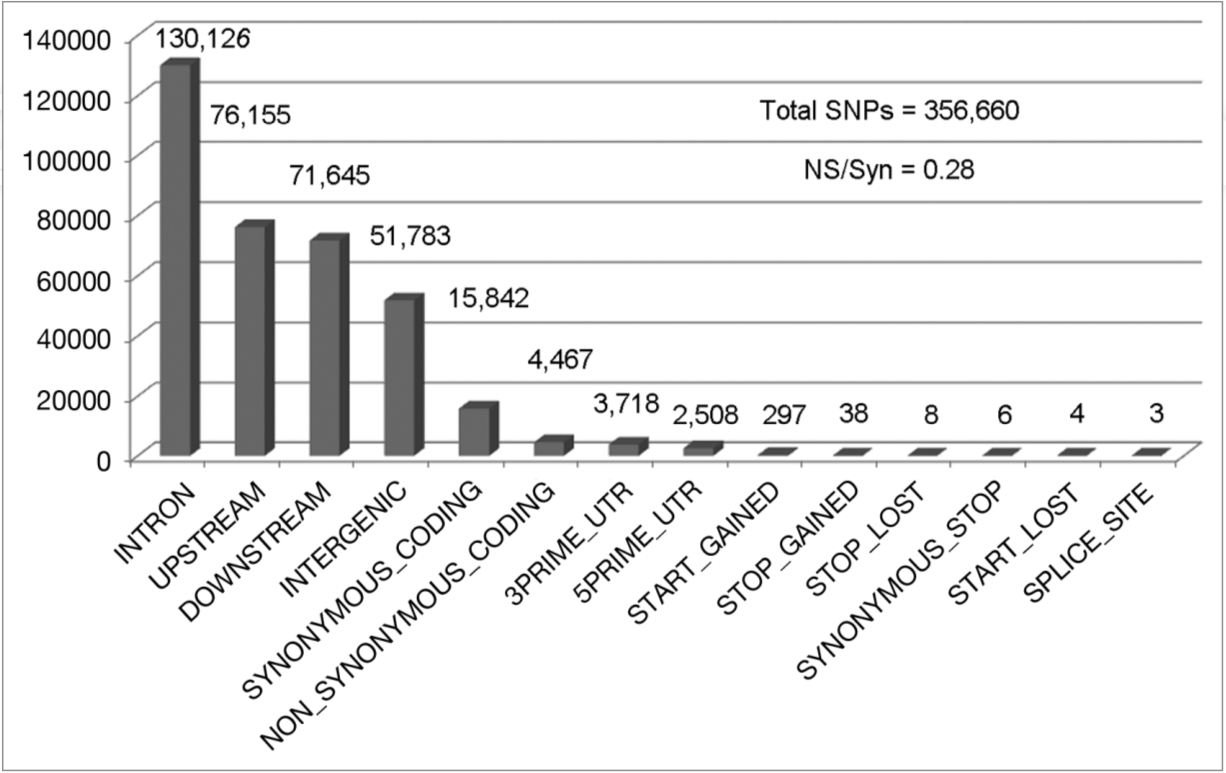
\includegraphics[width=14cm]{snpeff_fig1.png}
    \caption{Classification of SNPs in $w^{1118}$ ; iso-2; iso-3. The number of NSPs in each class is shown above the bar. The quality score was arbitrarily set at 70 and above for this graph.}
    \label{fig:snpeffTab3}
\end{figure}

An example of an essential protein-coding gene in Category 4, where the novel C-terminus is not conserved outside the Drosophila genus, is oceliless (oc), also known as orthodenticle (otd) (Fig. 3). The oc/otd gene has two in-frame stop-gained SNPs in $w^{1118}$ ; iso-2; iso-3. The oc/otd gene is a Hox-family transcription factor required for photoreceptor development in the compound eye and the light-sensing ocellus, embryonic development and brain segmentation. 23,24 The Hox domain is 60 amino acids, 59 of which are identical with the human Otd protein. The Hox domains, which arose before invertebrates and vertebrates split several hundred million years ago, are among the most conserved protein domains in bilaterally-symmetric organisms in evolution. 25 The two stop-gained SNPs are in the non-conserved C-terminal region of Oc/Otd, which is thought to have a transcriptional-regulatory function. Since both strains are viable, both oc/otd genes are apparently functional although they encode a protein with 489 amino acids in $w^{1118}$ ; iso-2; iso-3, and a protein with 543 amino acids in the reference genome (Table 6).

\begin{figure}
    \centering
    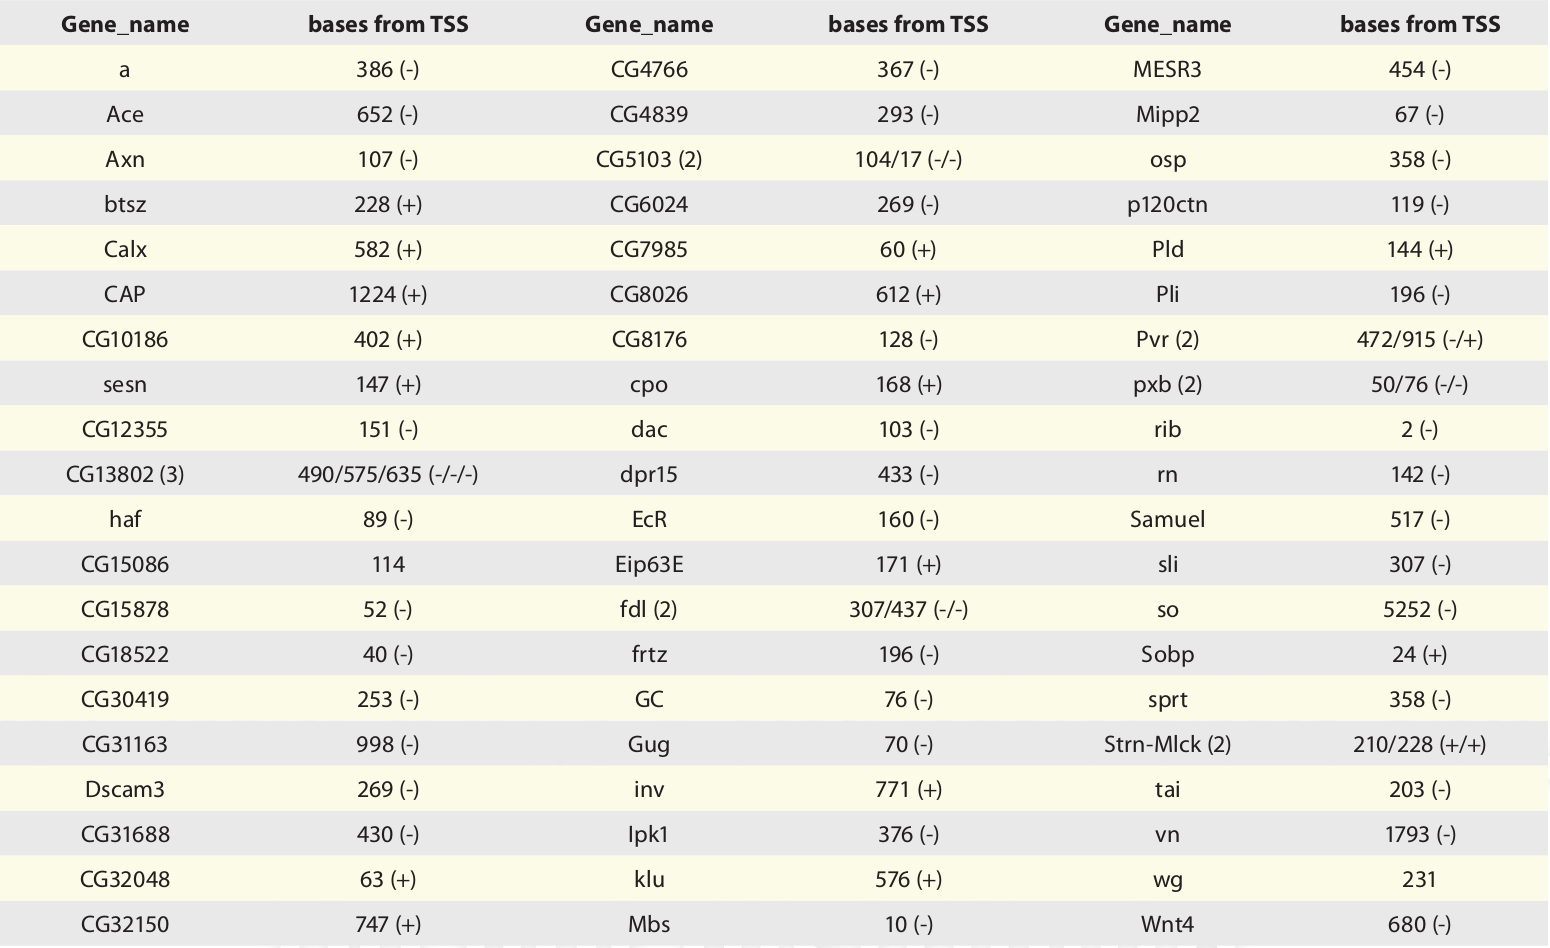
\includegraphics[width=14cm]{snpeff_table5.png}
    \caption{60 Genes with start-gaineded SNPs with ATGs. Bases from TSS, bases from translation start site not including the ATG start-gained SNP. (+), in same reading frame as annotated ATG. (-), in different reading frame as annotated ATG.}
    \label{fig:snpeffTab3}
\end{figure}

\begin{figure}
    \centering
    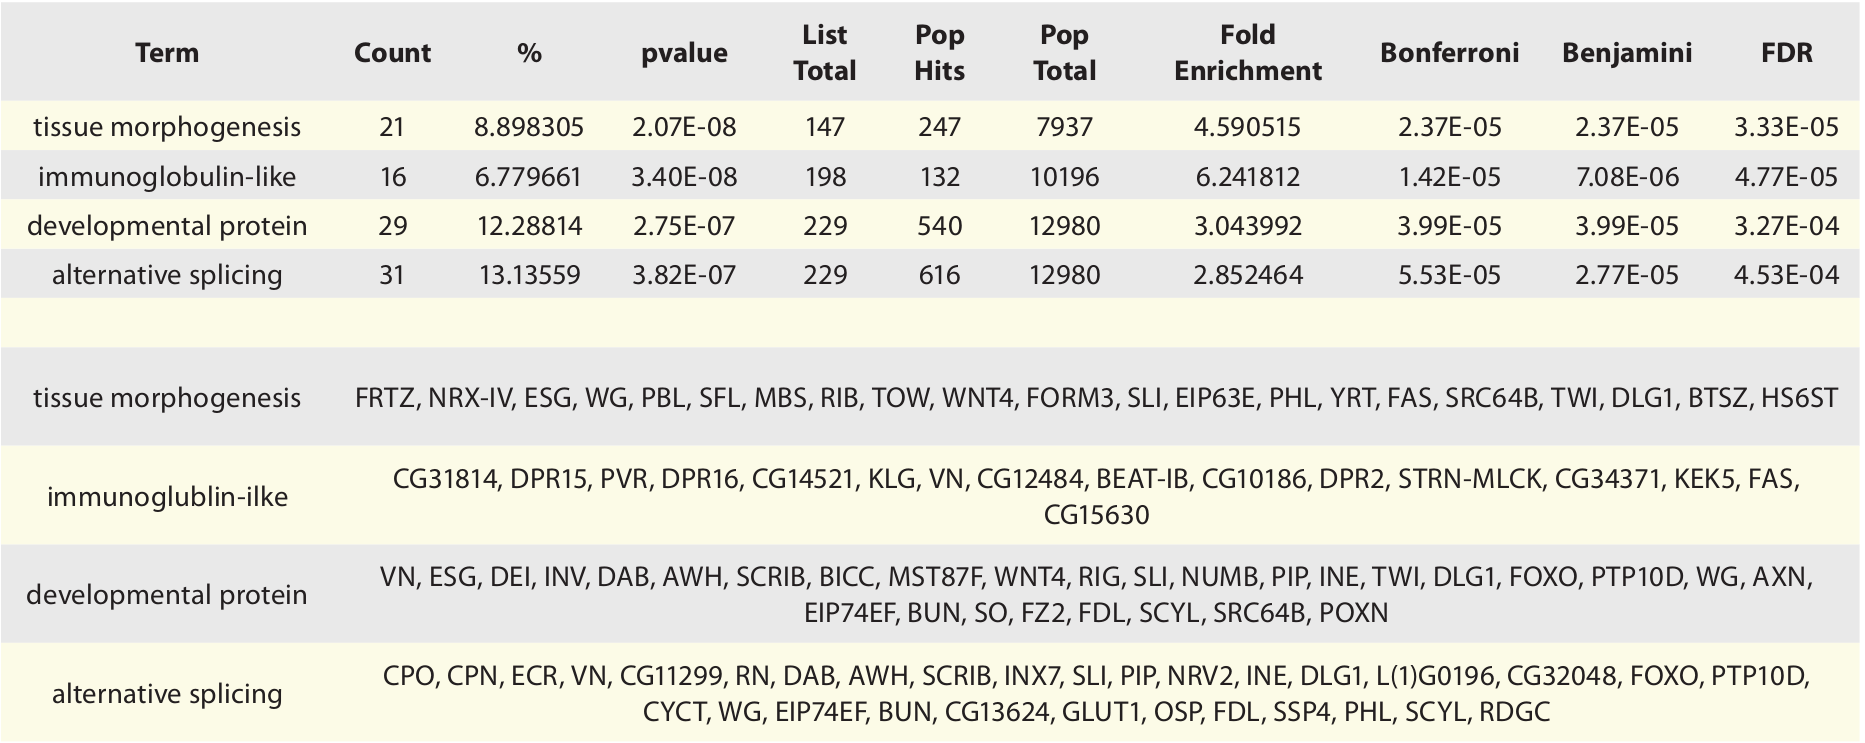
\includegraphics[width=14cm]{snpeff_table6.png}
    \caption{Genes with start-gained SNP GO categories in $w^{1118}$ ; iso-2; iso-3. Results of Gene ontology analysis for 297 start-gained SNPs in $w^{1118}$ ; iso-2; iso-3. Bottom, the genes in the indicated gene ontology category is listed.}
    \label{fig:snpeffTab3}
\end{figure}

An example of a stop-lost gene in class c, where the C-terminus is not conserved even among the Drosophila genera, is CG13958 that encodes a protein of unknown function (Fig. 4). In $w^{1118}$ ; iso-2; iso-3, CG13958 encodes a protein of 48 amino acids but in the reference genome it encodes a protein with 84 amino acids.  When BLASTp was done with the non-redundant (nr) data set, there was not much homology beyond the 38 th amino acid within the Drosophila genus. However, there was a near perfect (37/38) identity of the first 38 amino acids in four other Drosophila species: Drosophila grimshawi, Drosophila yakuba, Drosophila erecta and Drosophila virilus (Fig. 4). This protein likely arose in the Drosophila genus since it has no known homologs outside of this genus.

There are also five stop-lost SNPs in $w^{1118}$ ; iso-2; iso-3 (Table 6). All of these SNPs are in predicted protein-coding genes, metabotropic GABA-B receptor subtype 1 (GABA-B-R1), CG13958, CG4975, brown (bw), and POU domain motif 3 (pdm3). It is not known whether any of the these genes are essential in Drosophila besides bw, which is not required for viability.  However, the metabotropic GABA-B receptor subtype 1 (GABAB-R1) gene is required for normal behavior in mice 26 and the ortholog is therefore likely also essential in Drosophila, although no phenotypic data are available (www.flybase.org). The bw gene is classic gene first described in 1921 by Waaler, 27 which causes the eyes to be brown rather than red and encodes an ATPase binding cassette (ABC) transporter. 28 The bw 1 mutation in the reference strain is a spontaneous allele with a 412-transposon repeat insertion, 29 which would have been missed in our nextgeneration sequencing data because the input sequence we analyzed contained only short-read sequences that mapped uniquely to the reference genome.

Not much is known about the functions of several genes with in-frame stop-gained SNPs. The pdm3 gene is expressed in the larval and adult nervous system, and it encodes a highlyconserved Hox domain, but no phenotypic data are available (www.flybase.org). No phenotypic data are available for either CG13958 or CG4975. The protein encoding CG13958 has no known conserved domain, and its peak expression is observed within 06–24 h of embryogenes, during early larval stages, at stages throughout the pupal period, and in the adult male (www.  flybase.org). The protein encoded by CG4975 has an Armadillolike helical domain and an Ataxin-10 domain and has expression in the hind gut during the late larval and periods (www.flybase.  org). 30

\begin{figure}
    \centering
    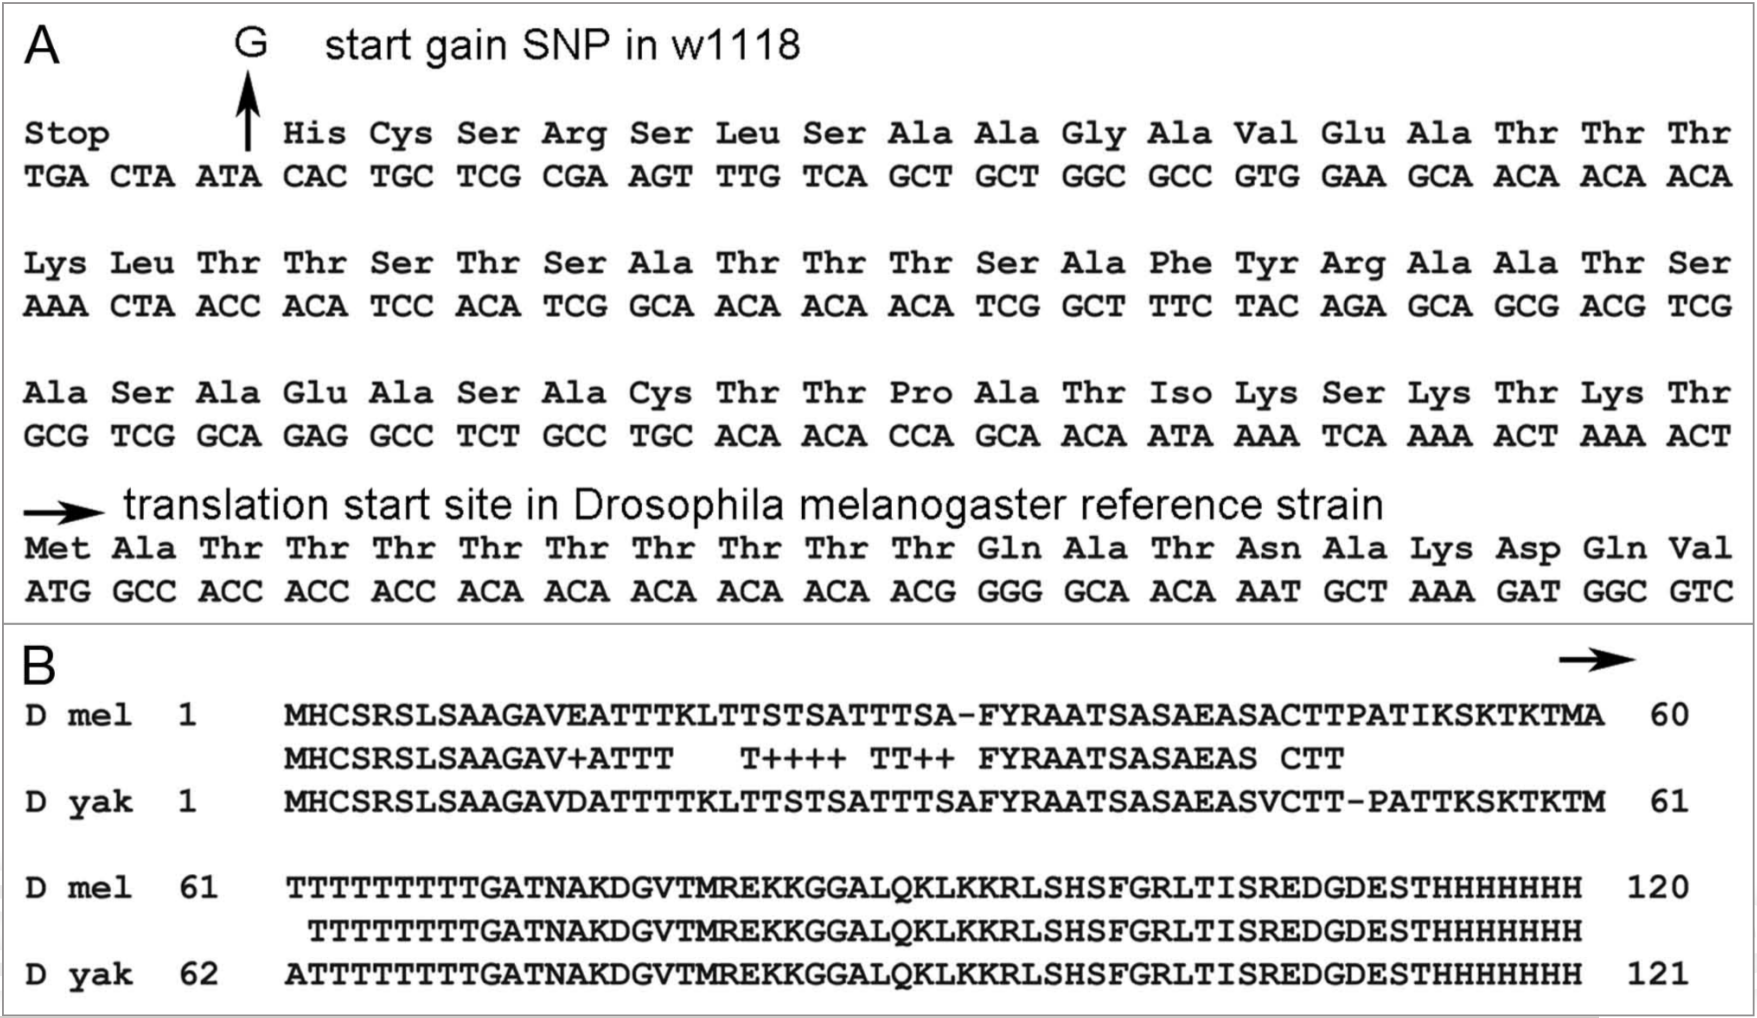
\includegraphics[width=14cm]{snpeff_fig2.png}
    \caption{Analysis of Eip63E start-gained SNP in $w^{1118}$ ; iso-2; iso-3. (A), Location of the start-gained SNP at the Eip63E locus. Notice that the reading frame is the same as the normal translation start site (TSS). (B), Conservation of 60 amino acid N-terminal region of Eip63E in $w^{1118}$ ; iso-2; iso-3 with Drosophila yakuba orthologous gene. The other sequenced Drosophila species do not have this N-terminal sequence (not shown).}
    \label{fig:snpeffTab3}
\end{figure}

Some of the stop-lost SNPs have interesting consequences. For example, a stop-lost SNP in $w^{1118}$ ; iso-2; iso-3 is in the CG13958 gene and causes an extension of eight amino acids before the next stop codon in 3' UTR sequence is reached (Fig. 5). Since the C-termini of CG13958 vary in $w^{1118}$ ; iso-2; iso-3 and the reference strains of Drosophila melanogaster, it is conceivable that the C-terminus might also fluctuate in other Drosophila species. To test this idea, we investigated the C-terminal regions of CG13958 homologs in other Drosophila species.

\begin{figure}
    \centering
    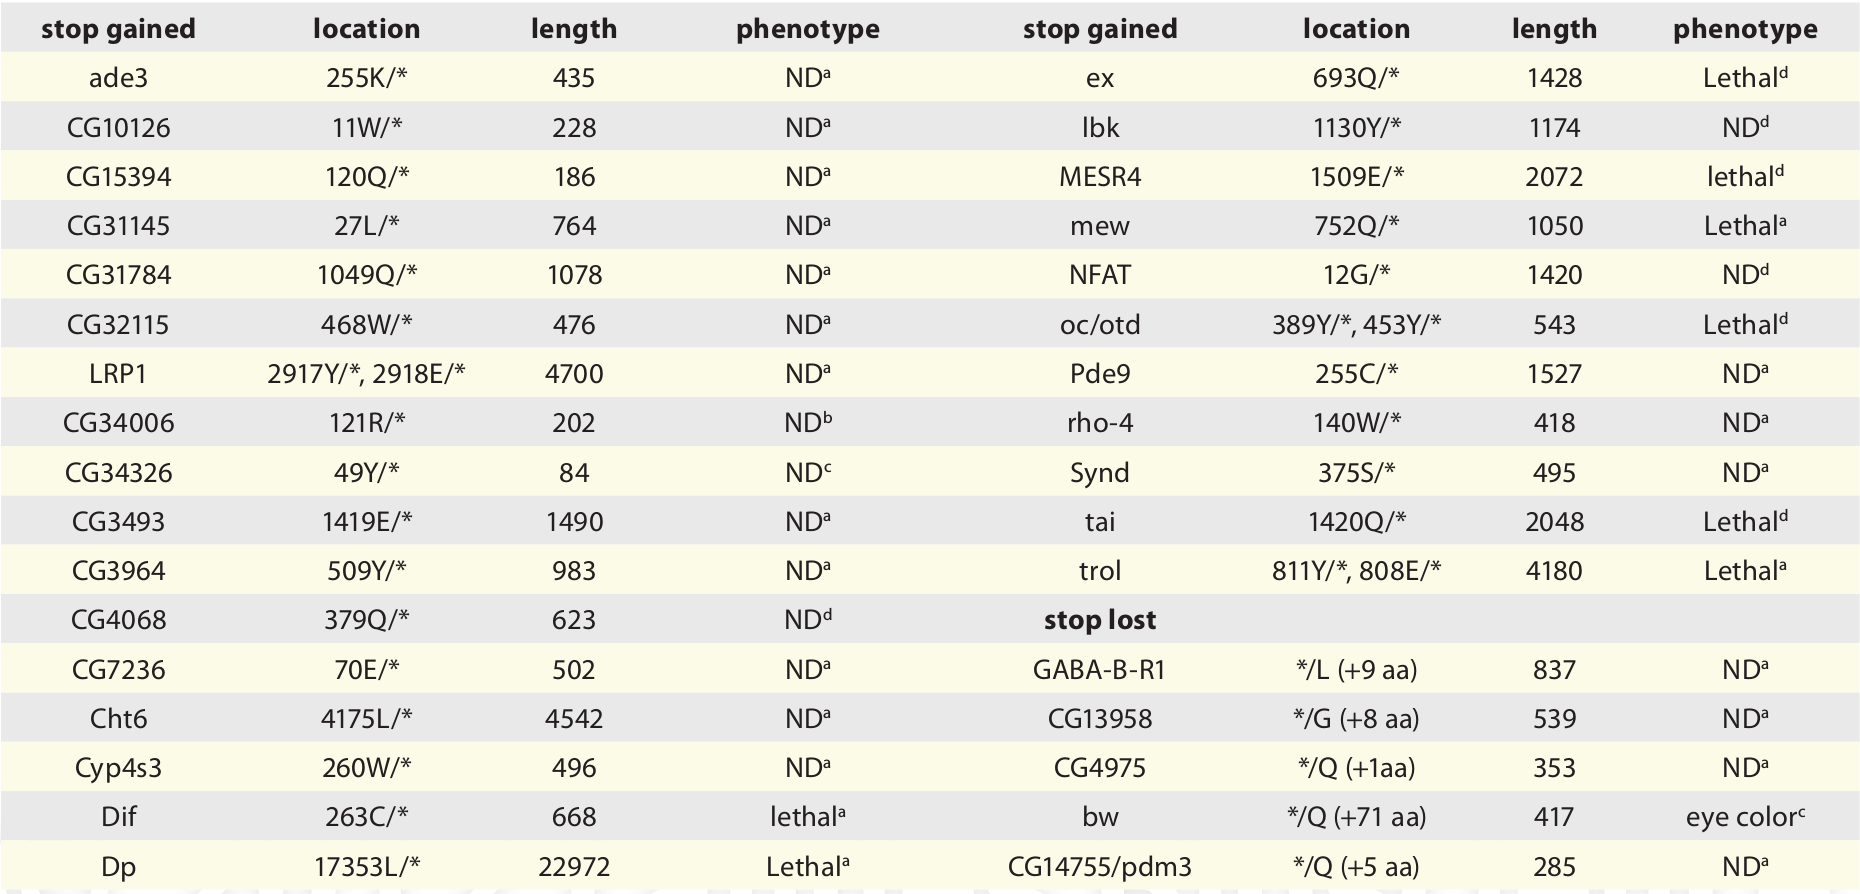
\includegraphics[width=14cm]{snpeff_table7.png}
    \caption{Stop gained and stop lost in $w^{1118}$ ; iso-2; iso-3. Stop gained, gene with stop gained SNP. Location, amino acid number changed to a stop codon (e.g., 255K/*, indicates lysine at amino acid changed to a stop codon). Length, the length of the protein in amino acids. Phenotype, not determined (ND), withdrawn (no longer considered a gene by FlyBase), and NPC (non-protein coding, such as a rRNA). For stop lost SNPs (bottom), */L (+9 aa) indicates that the next in frame stop is after nine additional amino acids are added. a-d refer to SNP categories 1–4 (see text).}
    \label{fig:snpeffTab3}
\end{figure}

We found that CG13958 homologs have variable C-terminal amino acids in different species of Drosophila. When the CG13958 protein is analyzed by protein Basic Local Alignment Search Tool (BLASTp) with the non-redundant (nr) protein database (http://www.ncbi.nlm.nih.gov/), at least two Drosophila species have extended C-terminal amino acids and at least three Drosophila species have missing amino acids at the C-termini (Fig. 5). For example, Drosophila pseudoobscura has three of the extended amino acids found in $w^{1118}$ ; iso-2; iso-3 and Drosophila mojavenais has four of them. In contrast, Drosophila simulans is missing the last terminal amino acid, Drosophila erecta is missing the last two terminal amino acids, and Drosophila yakuba is missing the last three amino acids found in the reference strain (Fig. 5). The large number of stop-gain and stop-lost SNPs in Drosophila likely has important implications on the evolution of protein function (see Discussion).

\begin{figure}
    \centering
    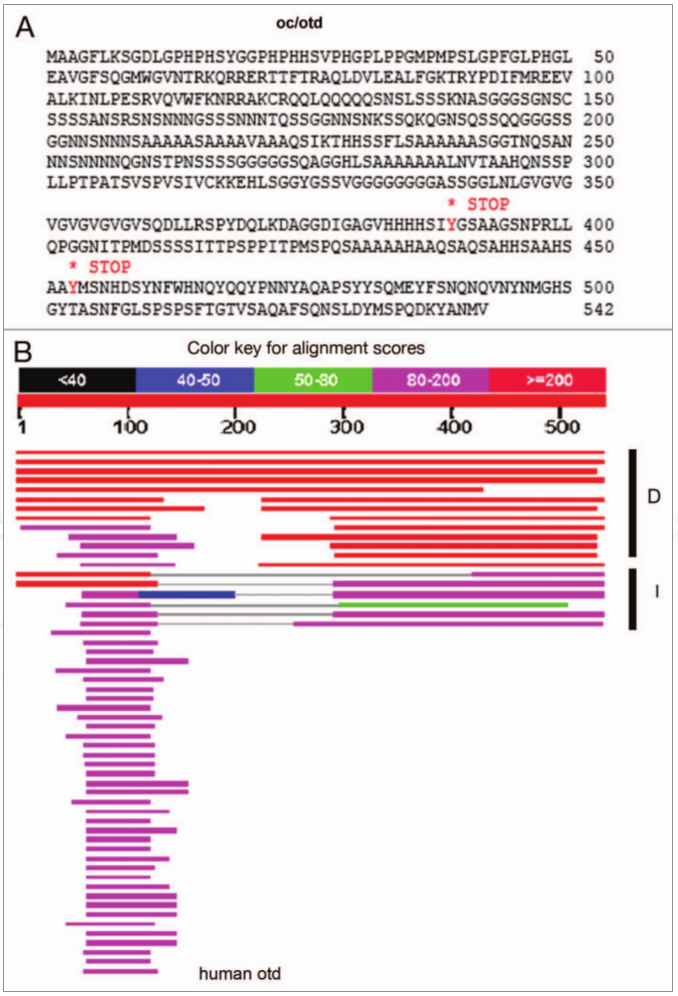
\includegraphics[width=14cm]{snpeff_fig3.png}
    \caption{Oc/Otd has two stop-gained SNPs in $w^{1118}$ ; iso-2; iso-3. (A) Location of the two stop gained SNPs in oc/otd. (B) Protein BLAST of Oc/Otd against the non-redundant (nr) protein database shows that only the 60 amino Hox domain flanking amino acid 100 is conserved from Drosophila to humans. The color coding shows the alignment scores.}
    \label{fig:snpeffTab3}
\end{figure}

Synonymous and non-synonymous SNPs in $w^{1118}$ ; iso-2; iso-3. There are 15,842 synonymous SNPs and 4,467 nonsynonymous SNPs in annotated coding regions in $w^{1118}$ ; iso-2; iso-3 (Fig. 1). A synonymous SNP (silent SNP) is defined as a SNP that does not change the amino acid in the protein, whereas a nonsynonymous SNP does. The genome-wide normalized N/S ratio (dN/dS), also called ω (i.e., ω = dN/dS), is by definition normalized to 1 in most evolutionary studies. 31 The non-normalized N/S ratio is \~0.28 in $w^{1118}$ ; iso-2; iso-3 compared with the reference genome, y 1 ; cn 1 bw 1 sp 1 (i.e., N/S = 4,467/15,842; Table 1).

We examined the distribution of synonymous and nonsynonymous SNPs genome-wide for $w^{1118}$ ; iso-2; iso-3 and saw higher levels of both classes of SNPs in the middle of the chromosome arms and lower levels near the centromeres and telomeres (Fig.  6 and left). This was expected because the number of SNPs is proportional to the recombination frequencies in the different regions of the chromosomes. 32,33 Also, our previous analyses of the distribution of total SNPs revealed a similar pattern. 1 We observed higher N/S ratios near the telomeres and centromeres and lower N/S ratios in the middle of the chromosome arms (Fig.  6 and right).

%---
\section{Discussion}
%---

In this paper, we used SnpEff to categorize the \~356,660 SNPs in $w^{1118}$ ; iso-2; iso-3 and place them into 14 different classes based on their predicted effects on protein function. In order of prevalence, these 14 classes are intron, upstream, downstream, intergenic, synonymous, non-synonymous, 3' UTR, 5' UTR, start-gained, stop-gained, stop-lost, synonymous-stop, start-lost and splice-site SNPs (Fig. 1). The reason for cataloging the SNPs in $w^{1118}$ ; iso2; iso-3 is to get a better appreciation of evolution of genome sequences and genome organization in this common laboratory strain. We appreciate the fact that both $w^{1118}$ ; iso-2; iso-3 and y 1 ; cn 1 bw 1 sp 1 are derived and highly manipulated laboratory strains and do not represent natural populations. Therefore, we do not mean to imply that the analyses in this paper are significant but rather just observational. To be meaningful, these observations need to be followed up with natural populations. Hundreds of Drosophila natural populations have already been or are in the process of being sequenced, so this should be feasible in the near future with a program such as SnpEff. 34

Many of the stop-gained and stoplost SNPs in $w^{1118}$ ; iso-2; iso-3 occur in essential genes that apparently still function after amino acid truncations caused by the stop-gained SNPs (Table 6). These non-critical effects of the stop-gained SNPs are worth noting because nonsense codons in the transcribed mRNAs generally result in nonfunctional protein products. For example, some genetic disorders, such as thalassemia and Duchenne muscular dystrophy (DMD), result from nonsense SNPs. 35-37 Also, nonsense SNP-mediated RNA decay exists in yeast, Drosophila and humans, and usually ensures that mRNAs with premature stop codons are degraded. 38

The stop-gained and stop-lost SNPs in essential genes, if they are validated, could have profound evolutionary implications and suggest the involvement of prions, analogous to [$PSI^+$], in the retention and selection of these SNPs.  Brian Cox, a geneticist working with the yeast Saccharomyces cerevisiae, discovered [$PSI^+$] in 1965 as a non-genetically transmissible trait with a cytoplasmic pattern of inheritance similar to mitochondria. 39 He isolated a yeast strain auxotrophic for adenine due to a nonsense mutation is able to survive in media lacking adenine when [$PSI^+$] is present. 39 Reed Wickner showed in 1994 that [$PSI^+$] resulted from a prion form of the translation termination factor, Sup35. 40 Lindquist and colleagues showed in 2008 that the [$PSI^+$] prion provides survival advantages in several stressful environments, such as high salt conditions. 41 They have speculated that Sup35 is an evolutionary capacitor that, when inactivated in the $PSI^+$ form, releases cryptic genetic variation that allow expression of novel C-terminal amino acids in hundreds of proteins, some of which are beneficial in stressful environments. 

How might prions be involved in revealing cryptic genetic variation in the 5' and 3' UTRs? While most prions are thought to not directly mutate DNA sequences, they could provide an environment that would make the retention and selection of beneficial SNPs more likely. For example, a stop-lost SNP would allow a modified protein with the new C-terminal tail to be always expressed, even when the prion is lost. 41 Therefore, a stop-lost SNP would more likely occur in a strain with beneficial codons in the 3' UTR because the cryptic C-terminal amino acids encoded by these nucleotides would provide a selective advantage in stressful (i.e., [$PSI^+$]) environments when they are translated.

\begin{figure}
    \centering
    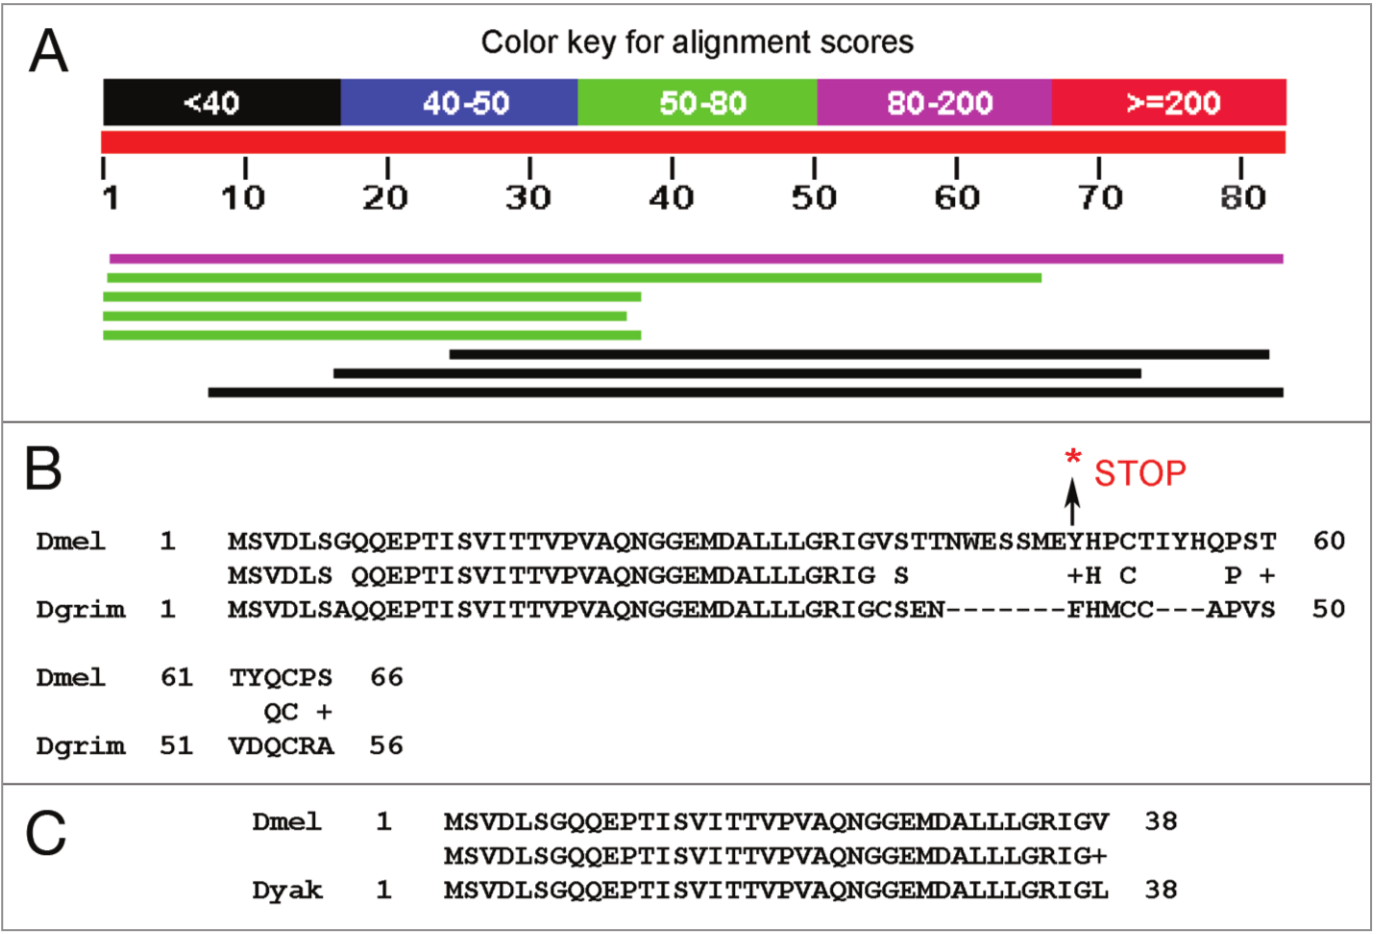
\includegraphics[width=14cm]{snpeff_fig4.png}
    \caption{
CG34326 has one stop-gained SNP in $w^{1118}$ ; iso-2; iso-3 in the non-conserved C-terminal region. (A) Protein BLAST of CG34326 against the non-redundant (nr) protein database shows that only the 38 N-terminal amino acids are conserved among Drosophila species and not beyond Drosophila. The colored lines represent the homologs from the following organisms: Drosophila melanogaster, Drosophila grimshawi, Drosophila yakuba, Drosophila erecta, Drosophila virilus, Ixodes
scapularis, Ixodes scapularis and Nycticebus coucang. (B) Aligment of Drosophila melanogaster CG34326 with orthologous gene from Drosophila grimshawi. (C) Aligment of Drosophila melanogaster CG34326 with orthologous gene from Drosophila yakuba.}
    \label{fig:snpeffTab3}
\end{figure}

It is attractive to speculate that a similar prion-mediated evolutionary mechanism might occur in Drosophila, for both stoploss and stop-gained SNPs, and that this might help explain the large number of SNPs that we see in these categories. We note that Drosophila has several Sup35 orthologs, some of which have N-terminal repeats that are known to be potentially prion-forming domains. 41 We acknowledge that this is a highly speculative explanation for the high numbers of start-gained and stop-lost SNPs, but we believe that it is worthy of further investigation.

The many potential start-gained SNPs in Drosophila might also have evolutionary implications. Similar to the cryptic genetic variation that is revealed by stop-lost mutations in the 3' UTR, start-gained SNPs reveal cryptic genetic variation in the 5' UTR. Uncovering the cryptic genetic variation in times of environmental stress, such as by inducing transcription initiation at start sites upstream of the normally-used transcription start sites, could be one mechanism to facilitate the use of potential start-gained SNPs. Further mutations and selection of the potential start-gained SNPs, such as by introducing better Kozak consensus sequences or more commonly used 5'-AUG-3' translation initiation codons, can stabilize the cryptic genetic variation further if it leads to improved survival or reproductive fitness in a stressful environment. While amino acid extensions and deletions in known essential genes occur only 8 times in $w^{1118}$ ; iso-2; iso-3 compared with the reference strain (Table 7), as laboratories begin to sequence hundreds or even thousands of individuals in a population, extensions and deletions are likely to be found in a large proportion of functional genes.

\begin{figure}
    \centering
    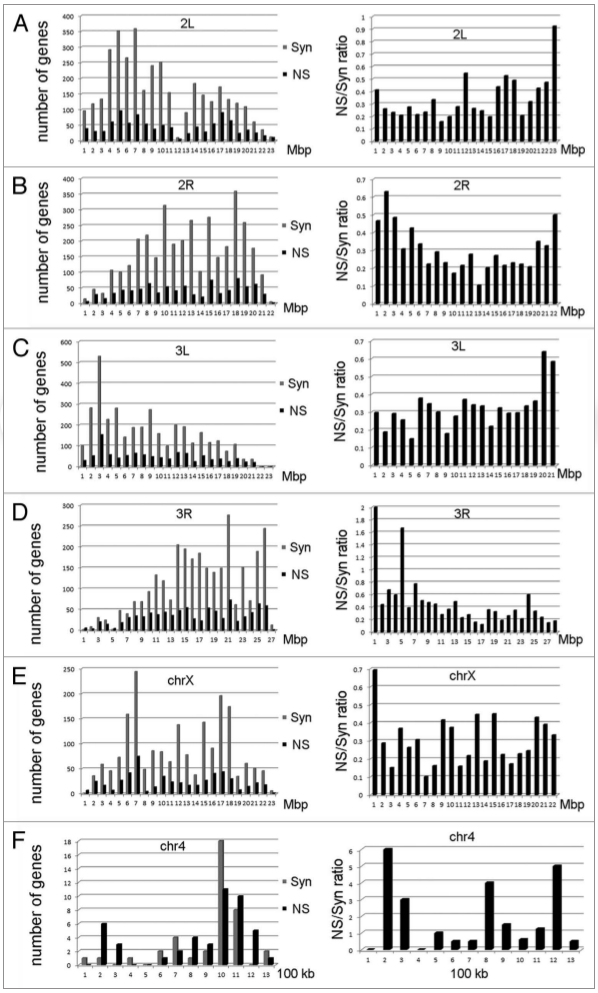
\includegraphics[width=14cm]{snpeff_fig6.png}
    \caption{Nonsynonymous to synonymous ratios along the chromosome arms in $w^{1118}$ ; iso-2; iso-3. (A) Left, Nonsynonymous SNPs at 1 Mbp intervals along the 2L chromosome arm (black) and synonymous SNPs (gray). Right, N/S ratios (NS/Syn) along the chromosome arms. Notice that N/S ratios are higher near the centromere and telomere (see text). (B–F) as in (A), but for chromosome arms 2R, 3L, 3R, 4 and X.}
    \label{fig:snpeffTab3}
\end{figure}

Finally, we recently upgraded SnpEff further by including over 320 databases for different reference genome versions that can be analyzed (http://snpeff.  sourceforge.net/SnpSift.html). Sources of information for creating these databases are ENSEMBL, UCSC Genome Bioinformatics website as well as organism specific databases, such as FlyBase (Drosophila melanogaster), WormBase (C.  elegans) and TAIR (Arabidopsis thaliana), to name a few. The program SnpEff is open access and additional genomes can be added and assistance in using SnpEff can be provided upon request. Rapid analyses of whole-genome sequencing data should now be feasible to perform by any laboratory

%---
\section{Methods}
%---

\textbf{SnpEff overview.} The program is divided in two main parts (i) database build and (ii) effect calculation. Part (i) Database build is usually not run by the user, because many databases containing genomic annotations are available. Databases are build using a reference genome, a FASTA file, and an annotation file, usually GTF, GFF or RefSeq table, provided by ENSEMBL, UCSC Genome Bioinformatics website or other specific websites, such as FlyBase, WormBase and TAIR. SnpEff databases are gzip serialized objects that represent genomic annotations.

Part (ii) Effect calculations can be performed once the user has downloaded, or built, the database. The program loads the binary database and builds a data structure called ``interval forest," used to perform an efficient interval search (see next section). Input files, usually in VCF format, are parsed and each variant queries the data structures to find intersecting genomic annotations. All intersecting genomic regions are reported and whenever these regions include an exon, the coding effect of the variant is calculated (hence the name of the program). A list of the reported effects and annotations is shown in Table 2, additional information produced by the program, is shown in Table 3 and Table 4, for different output formats.

\textbf{SnpEff algorithms.} In order to be able to process thousands of variants per second, we implemented an efficient data structure that allows for arbitrary interval overlaps. We created an interval forest, which is a hash of interval trees indexed by chromosome.  Each interval tree 42 is composed of nodes. Each node has five elements (i) a center point, (ii) a pointer to a node having all intervals to the left of the center, (iii) a pointer to a node having all intervals to the right of the center, (iv) all intervals overlapping the center point sorted by start position and (v) all intervals overlapping the center point, sorted by end position.

Querying an interval tree requires O (log n + m) time, where n is the number of intervals in the tree and m is the number of intervals in the result. Having a hash of trees, optimizes the search by reducing the number of intervals per tree.

In order to create this the interval forest, genomic information can be parsed from three main annotation formats: GTF (version 2.2), GFF (versions 3 and 2), UCSC Genome Bioinformatics website RefSeqTables and tab separated text files (TXT). Once the interval forest is created, the structure is serialized and compressed (GZIP) into a binary database. There are over 250 genomic binary databases that are currently distributed with SnpEff, which include all genomes from ENSEMBL.

\begin{figure}
    \centering
    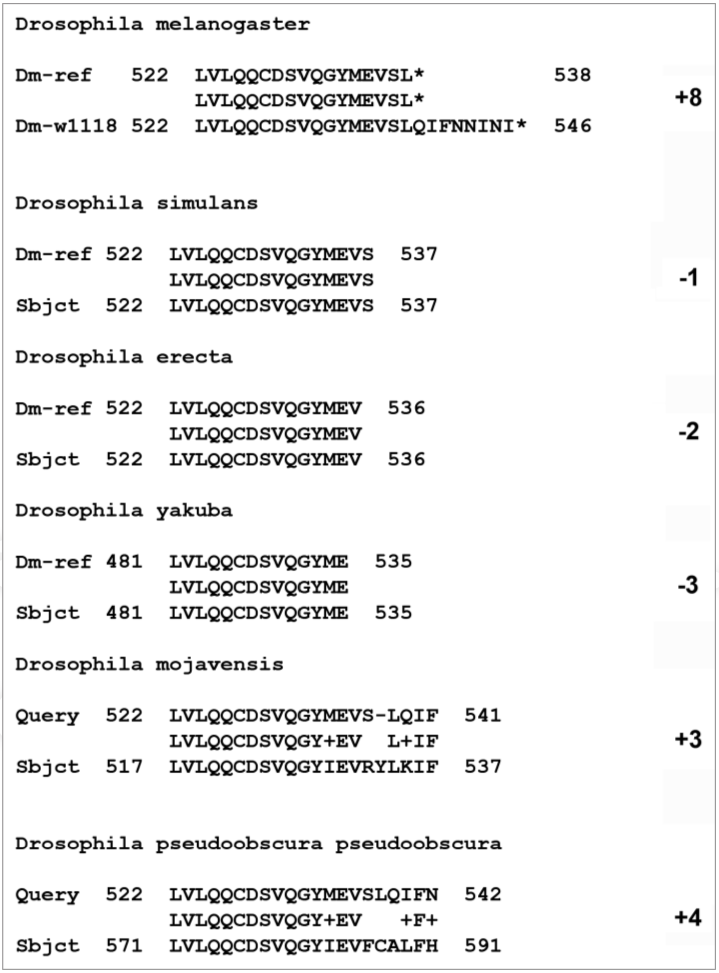
\includegraphics[width=14cm]{snpeff_fig5.png}
    \caption{CG13958 has a stop lost SNP in w 1118 ; iso-2; iso-3. The top comparison shows the alignment of the Drosophila melanogaster reference genome with $w^{1118}$ ; iso-2; iso-3. Notice that the stop lost causes an extension of 9 amino acids. The second through sixth comparisons shows the alignment of Drosophila simulans, Drosophila erecta, Drosophila yakuba, Drosophila mojavensis and Drosophila pseudoobscura pseudoobscura (Sbjct) with the Drosophila melanogaster reference genome (Dm-ref). The number of terminal amino acids missing or gained is shown (-1 to +3). }
    \label{fig:snpeffTab3}
\end{figure}

\textbf{SnpEff accuracy.} As part of our standard development cycle, we perform accuracy testing by comparing SnpEff to ENSEMBL ``Variant effect predictor," which we consider it is the ``gold standard." Current unity testing includes over a hundred test cases with thousands of variants each to ensure predictions are accurate.

\textbf{SnpEff integration.} SnpEff provides integration with third party tools, such as Galaxy, 43 which creates a web based interface for bioinformatic analysis pipelines.  Integration with Genome analysis tool kit 4 (GATK) was provided by the GATK team.  Detailed information on how to download, install and run, as well as usage examples of the program, can be found at http:/snpEff.sourceforge.net.  

Data access. SnpEff Data can be accessed from the Supplemental data file for $w^{1118}$ ; iso-2; iso-3 or by contacting D.M.R.

Disclosure of Potential Conflicts of Interest No potential conflicts of interest were disclosed.


%---
\section{Acknowledgements}
%---

This work was supported by a Michigan Core Technology grant from the State of Michigan’s 21 st Century Fund Program to the Wayne State University Applied Genomics Technology Center. This work was also supported by the Environmental Health Sciences Center in Molecular and Cellular Toxicology with Human Applications Grant P30 ES06639 at Wayne

State University, NIH R01 grants (ES012933) to D.M.R. and DK071073 to X.L. We thank David Roazen, Eric Banks and Mark DePristo in the GATK team at the Broad Institute who integrated SnpEff with the Genome Analysis Toolkit (GATK).

Note Supplemental material can be found at: http://www.landesbioscience.com/ journals/fly/article/19695

%---
\section{Epilogue}
%---

At the beginning of my Ph.D., functional annotation of genomic variants was an unsolved problem with many research labs creating in-house custom solutions that oftentimes were inefficient and lacking of rigorous testing. As a consequence, shortly after SnpEff \& SnpSift were released they quickly became widely adopted by the research community as well as many private organizations. Currently SnpEff \& SnpSift has over 250 downloads per week (as reported by  SourceForge, where the tools are hosted). So far SnpEff \& SnpSift  have been cited over 400 times.

\subsection{Data structures for annotations}

A very simple approach used by ANNOVAR \cite{wang2010annovar} is to create an index by dividing each chromosome into $N$ bins of equal size. All genomic features are stored in a hash table indexed by chromosome name and bin number. This approach has running time of $O(n)$ where $n$ is the number of features, but it can be easily tuned by creating small bins, at the cost of increased memory requirements.

Another approach \cite{cingolani2012program} is to use an ``interval forest'', which is a hash of ``interval trees'' indexed by chromosome. Each interval tree is composed of nodes. Each node has five elements i) a center point, ii) a pointer to a node having all intervals to the left of the center, iii) a pointer to a node having all intervals to the right of the center, iv) all intervals overlapping the center point sorted by start position, and v) all interval overlapping the center point sorted by end position. Querying an interval tree requires $O[log(n) + m]$ time, where $n$ is the number of features in the tree and $m$ is the number of features in the result. Having a hash of trees optimizes the search by reducing the number of intervals per tree.
